\documentclass[9pt]{beamer}
\mode<presentation>{}
\usepackage{beamerthemesplit} 

\setbeamertemplate{footline}[frame number]
\setbeamertemplate{headline}{}

\usepackage[english]{babel}
\usepackage[utf8x]{inputenc}
\usepackage{xcolor}

\title[PPT - Autonomous Mission Planning for Unmanned Surface Vehicles..]{Autonomous Mission Planning for Unmanned Surface Vehicles Piloted by Multiple Specialized Agents Using Heuristic and Metaheuristic Techniques}
\author{Evan Krell}
\institute{Texas A\&M University - Corpus Christi}
\date{November 2018}

\begin{document}

\begin{frame}
  \titlepage
\end{frame}

\begin{frame}{Outline}
  \tableofcontents
\end{frame}

\section{Problem Description}

\begin{frame}{Problem Description}
    \begin{block}{Unmanned Surface Vehicles (USVs)}
	    \begin{itemize}
    	    \item Typically used with remote control or following manually-defined paths
    	    \item Would like to delegate responsibilities to intelligent, capable marine agents
        \end{itemize}
    \end{block}
    \begin{block}{Applications}
	    \begin{itemize}
    	    \item Scientific: surveying, monitoring, marine animal tracking	    
	        \item Commercial: shipping, underwater infrastructure imaging
	        \item Search \& rescue: marine disaster recovery
    	    \item Military: surveillance, reconnaissance, communications, demining, defence
        \end{itemize}
    \end{block}
    \begin{center}
        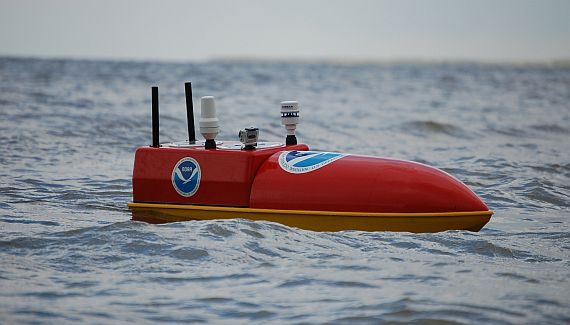
\includegraphics[width=0.7\textwidth,trim={1cm 2cm 1cm 1cm},clip]{img/EMILY_NOAA.jpg}
    \end{center}
\end{frame}

\begin{frame}{Problem Description}
    \begin{block}{Typical USV Missions}
        \begin{columns}
            \begin{column}{0.5\textwidth}
                \begin{block}{}
                    \begin{center}
                        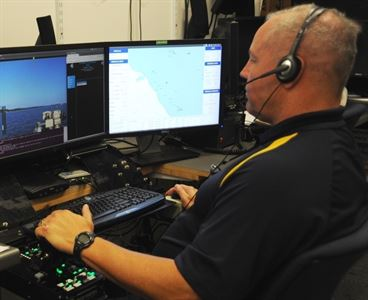
\includegraphics[width=\textwidth]{img/traditional.JPG}
                        \vline
                        \linebreak
                        Remote control of USV
                    \end{center}
                \end{block}
            \end{column}
            \begin{column}{0.5\textwidth}
                \begin{block}{}
                    \begin{center}
                        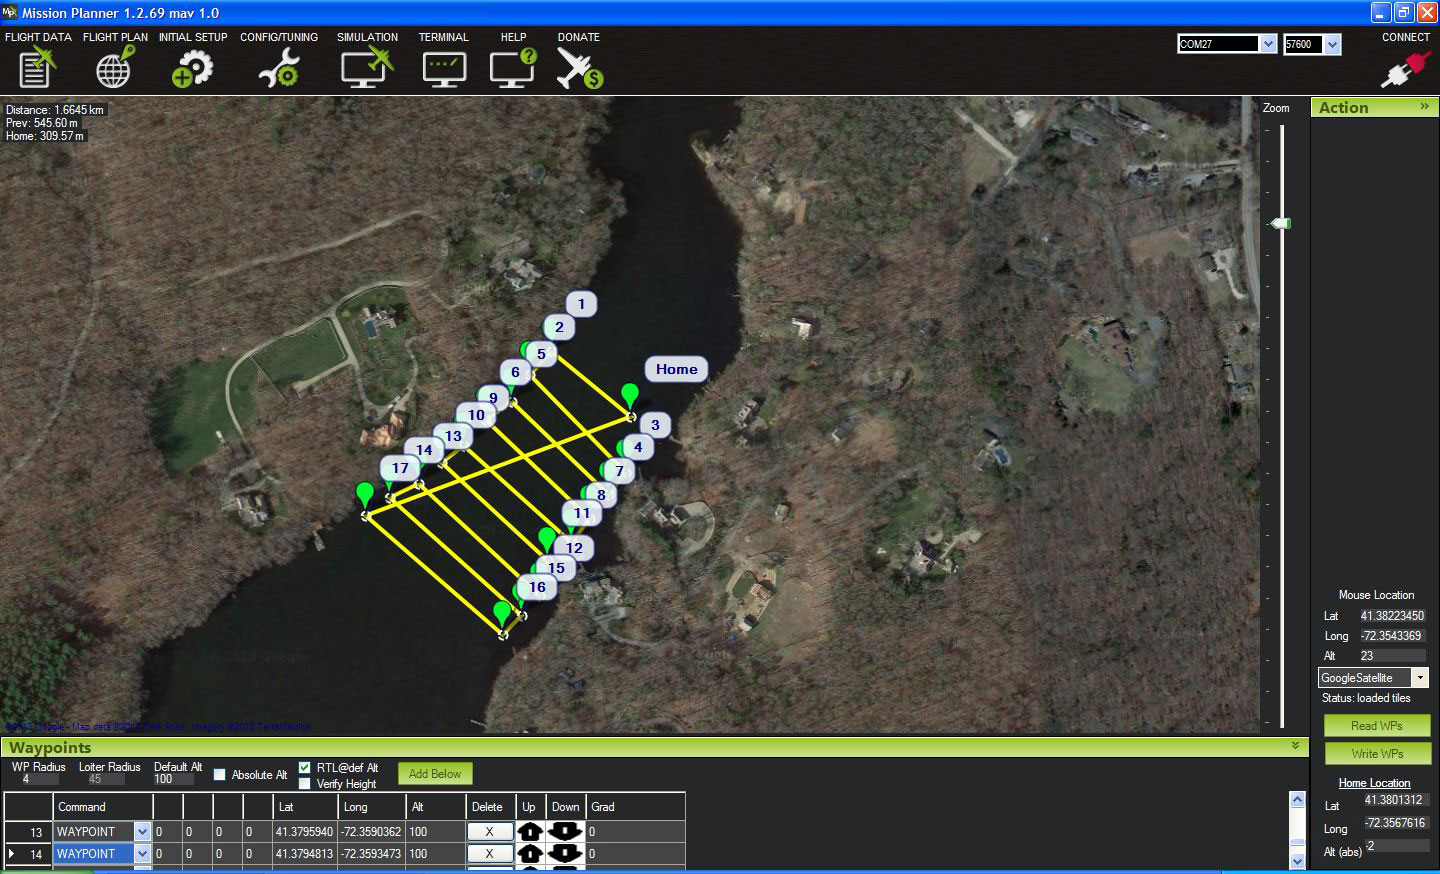
\includegraphics[width=\textwidth,trim={2cm 2cm 8cm 2cm},clip]{img/Jetyak4Waypoints.jpg}
                        \vline
                        \linebreak
                        Manually set waypoints for autopilot
                    \end{center}
                \end{block}
            \end{column}
        \end{columns}
    \end{block}
\end{frame}

\begin{frame}{Problem Description}
    \begin{block}{Challenges}
	    \begin{itemize}
    	    \item \textbf{Subject to complex dynamic environment}
    	    \item \textbf{Plans with computationally complex algorithms}
	        \item Requires awareness of above and below waterline
	        \item Sensing complicated by platform instability and high noise
    	    \item Must navigate among marine traffic
    	    \item Moves as nonholonomic, dynamic system with large turn radius
    	    \end{itemize}
    \end{block}
    \begin{center}
        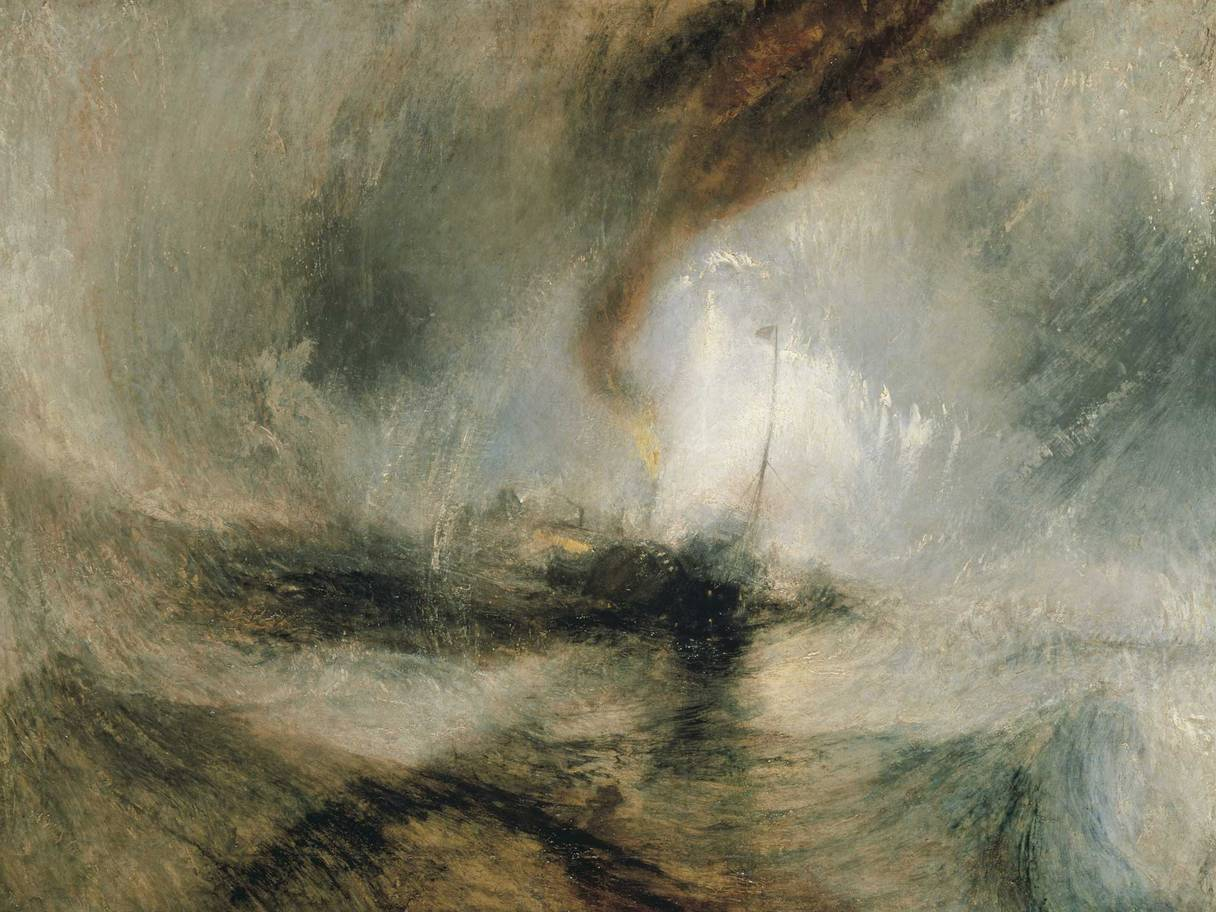
\includegraphics[width=0.5\textwidth,trim={5cm 5cm 4cm 4cm},clip]{img/turner_boat.jpg}
    \end{center}
\end{frame}


\section{Prior Work}
\begin{frame}{Prior Work}
    \begin{block}{Autonomous Navigation}
	    \begin{itemize}
    	    \item Guidance, navigation and control is well established with algorithms for path following (such as PurePursuit) and for state estimation (extended Kalman filter)
    	    \item Sensor imagery and reactive behaviors enable collision detection and avoidance
    	    \item Vehicles can be made to follow marine traffic rules and travel in formation
    	    \item Many systems include a \textit{follow} mode that can follow other vehicles, tagged animals, etc
        \end{itemize}
    \end{block}
    \begin{columns}
        \begin{column}{0.45\textwidth}
            \begin{block}{}
                \begin{center}
                    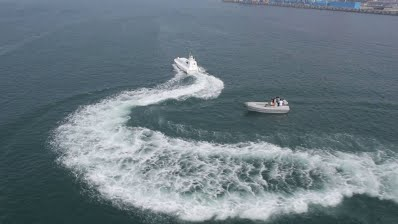
\includegraphics[width=0.7\textwidth,trim={5cm 1cm 2cm 1cm},clip]{img/collisionavoidance.jpg}

                    Collision avoidance 
                \end{center}
            \end{block}
        \end{column}
        \begin{column}{0.45\textwidth}
            \begin{block}{}
                \begin{center}
                    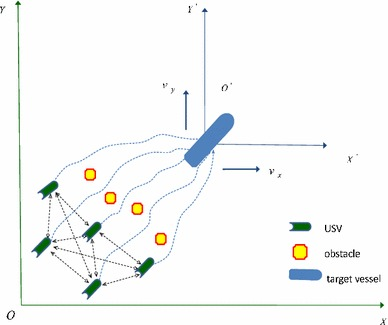
\includegraphics[width=0.7\textwidth,trim={1cm 1cm 4cm 3cm},clip]{img/formation.jpg}

                    Formation maneuver
                \end{center}
            \end{block}
        \end{column}
    \end{columns}
\end{frame}

\begin{frame}{Prior Work}
    \begin{columns}
        \begin{column}{0.45\textwidth}
            \begin{block}{Goto Path Planning}
                \begin{center}
                    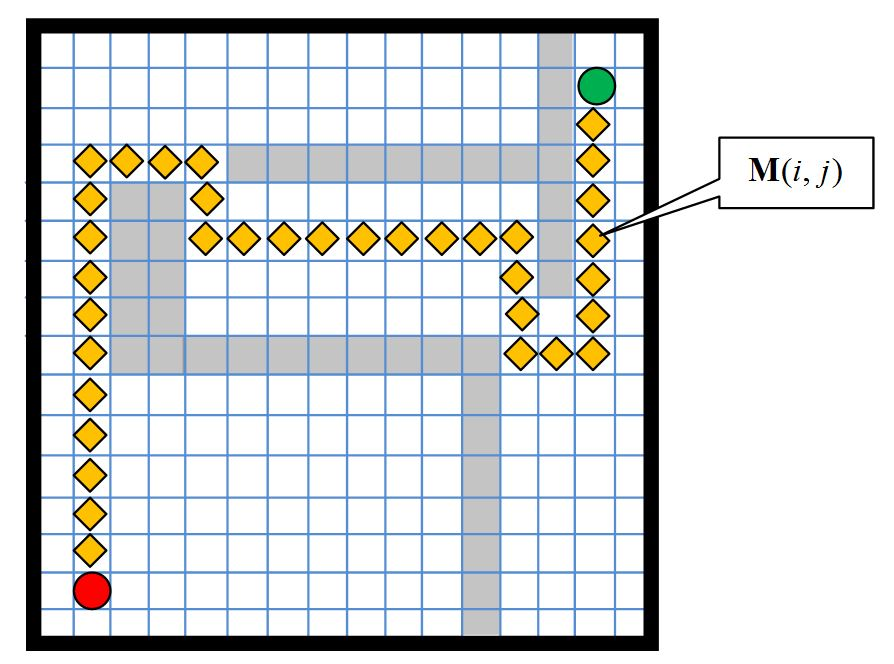
\includegraphics[width=\textwidth,trim={1cm 2cm 5cm 2cm},clip]{img/pathplanning.jpg}
                    \linebreak
                    Computationally complex, even using heuristic and metaheuristic algorithms. 
                    Much work has been done on this problem, but further complicated by dynamic marine environment.
                    Optimizing duration and energy instead of just distance. 
                \end{center}
            \end{block}
        \end{column}
        \begin{column}{0.45\textwidth}
            \begin{block}{Coverage Path Planning}
                \begin{center}
                    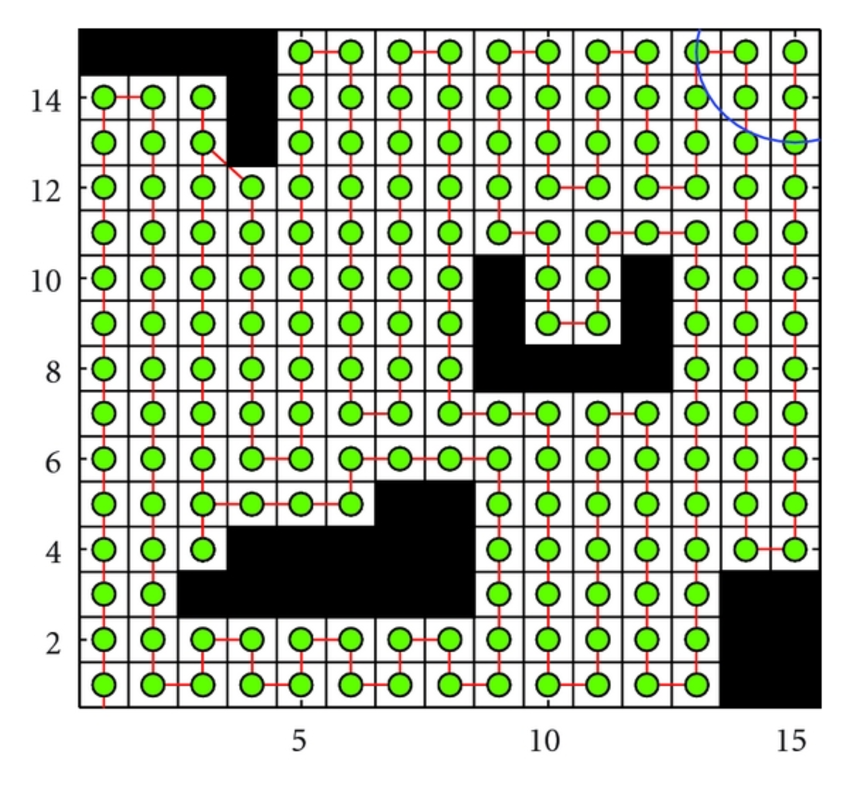
\includegraphics[width=0.85\textwidth,trim={1cm 2cm 2cm 1cm},clip]{img/coverageplanning.png}
                    \linebreak
                    More complicated since (1) a large number of waypoints to solve and (2) maximizing coverage is opposite to minimizing distance. Doing both is especially challenging for heuristic algorithms that may reach a local optimum.
                \end{center}
            \end{block}
        \end{column}
    \end{columns}
\end{frame}

\begin{frame}{Prior Work}
    \begin{block}{CaRACaS: Control Architecture for Robotic Agent Command and Sensing}
	    \begin{itemize}
	        \item US Navy's platform-agnostic coordinated mission planning system
    	    \item One of few that does onboard mission planning beyond path planning
            \item USVs equipped with the system are part of heterogeneous swarm
	        \item Tasks: Escort ships, protect areas, attack enemy ships
    	    \item Collision detection \& avoidance, COLREGS navigation
    	    \item Able to detect and react to perceived threats
    	    \item Integrated hardware and software
    	    \end{itemize}
    \end{block}
\end{frame}  

\begin{frame}{Prior Work}
    \begin{block}{CaRACaS: Control Architecture for Robotic Agent Command and Sensing}
        \begin{center}
            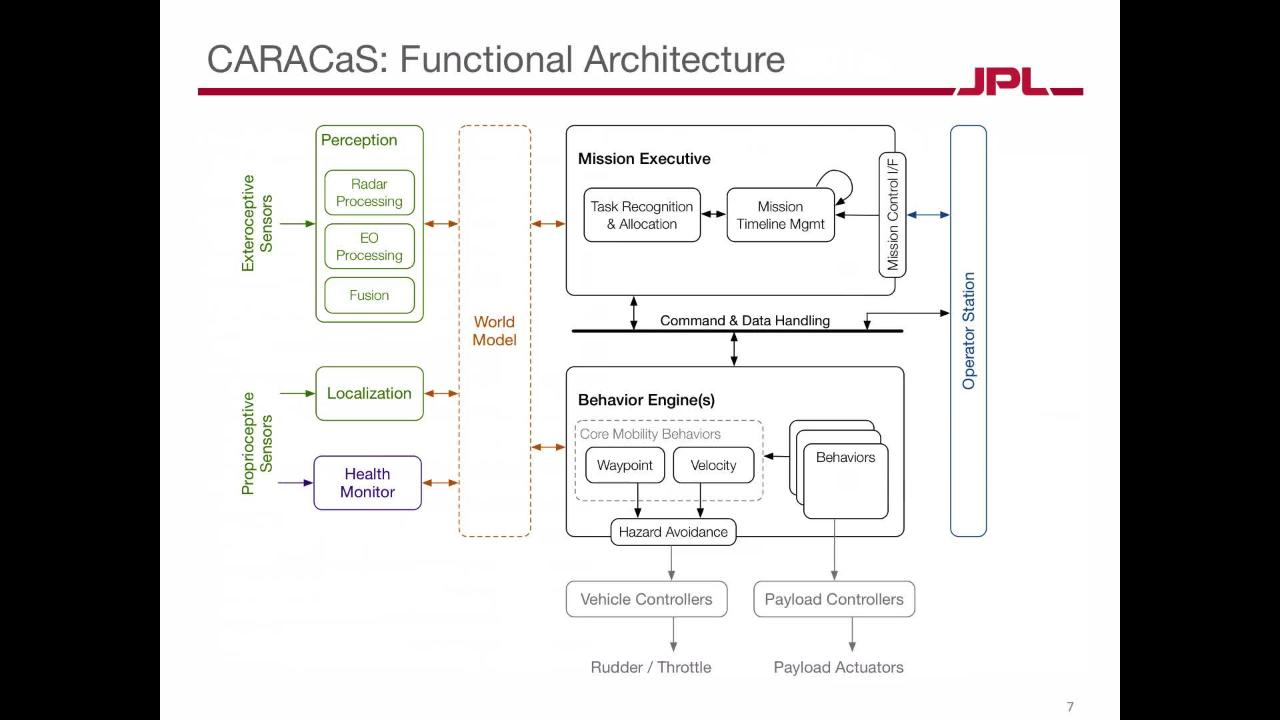
\includegraphics[width=\textwidth,trim={7cm 1cm 7cm 4cm},clip]{img/caracas.jpg}
        \end{center}
    \end{block}
\end{frame}

\begin{frame}{Prior Work}
    \begin{block}{Autonomous exploration, investigation, and setting objectives}
	    \begin{itemize}
	        \item Have seen systems where objectives are manually supplied or selected from predetermined reactions
    	    \item But want a USV with higher-level goals such as \textit{investigate Laguna Madre and alert if something interesting is found}
            \item Very little work in this area exists
	        \item Requires reliable mission planning and navigation
        \end{itemize}
    \end{block}
    \begin{columns}
        \begin{column}{0.50\textwidth}
            \begin{block}{JPL's Earth Observing-1}
                \begin{center}
                    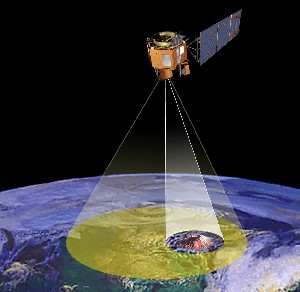
\includegraphics[width=0.75\textwidth,trim={0cm 0cm 0cm 0cm},clip]{img/eo1.jpg}
                \end{center}
            \end{block}
        \end{column}
        \begin{column}{0.50\textwidth}
            \begin{block}{}
                \begin{itemize}
	                \item \textit{Autonomous sciencecraft experiment}
    	            \item Onboard analysis: detect image characteristics to such as novel features or sudden change
                    \item Replans to focus on areas of interest
	                \item Prioritizes interesting data to send to earth first
                \end{itemize}
            \end{block}
        \end{column}
    \end{columns}
\end{frame}  


\section{Approach}

\begin{frame}{Approach}
    \begin{block}{Concept}
        Rather than a single integrated system, autonomy can be achieved using multiple specialized autonomous agents
    \end{block}
    \begin{columns}
        \begin{column}{0.33\textwidth}
            \begin{block}{Analyst}
                \begin{center}
                    \begin{itemize}
    	                \item Data analysis: detect features, change, classification
        	            \item Evaluation: assign scientific reward of visiting area 
                        \item Assign targets for \textit{Surveyer} agent
                    \end{itemize}
                    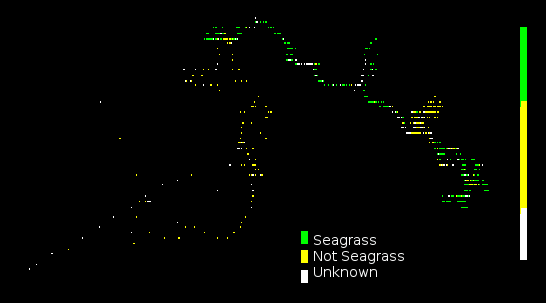
\includegraphics[width=0.75\textwidth,trim={6cm .5cm 4cm .5cm},clip]{img/seagrass.png}
                \end{center}
            \end{block}
        \end{column}
        \begin{column}{0.33\textwidth}
            \begin{block}{Surveyer}
                \begin{center}
                    \begin{itemize}
    	                \item Maximize number of visited targets
        	            \item Collect additional opportunistic reward
                        \item Optimize planning considering complex marine environment
                        \item Emphasize vehicle safety
                    \end{itemize}
                    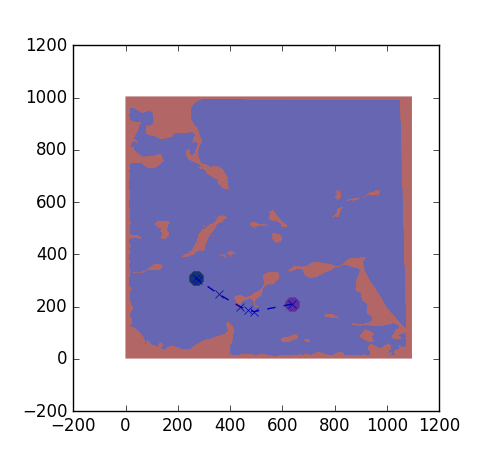
\includegraphics[width=0.75\textwidth,trim={4cm 2cm 4cm 6cm},clip]{img/samplepath.png}
                \end{center}
            \end{block}
        \end{column}
        \begin{column}{0.33\textwidth}
            \begin{block}{Navigator}
                \begin{itemize}
	                \item Path following (mission execution)
    	            \item Collision detection \& avoidance
                    \item Follow COLREGS
	                \item Any issuing of motor commands
                \end{itemize}
                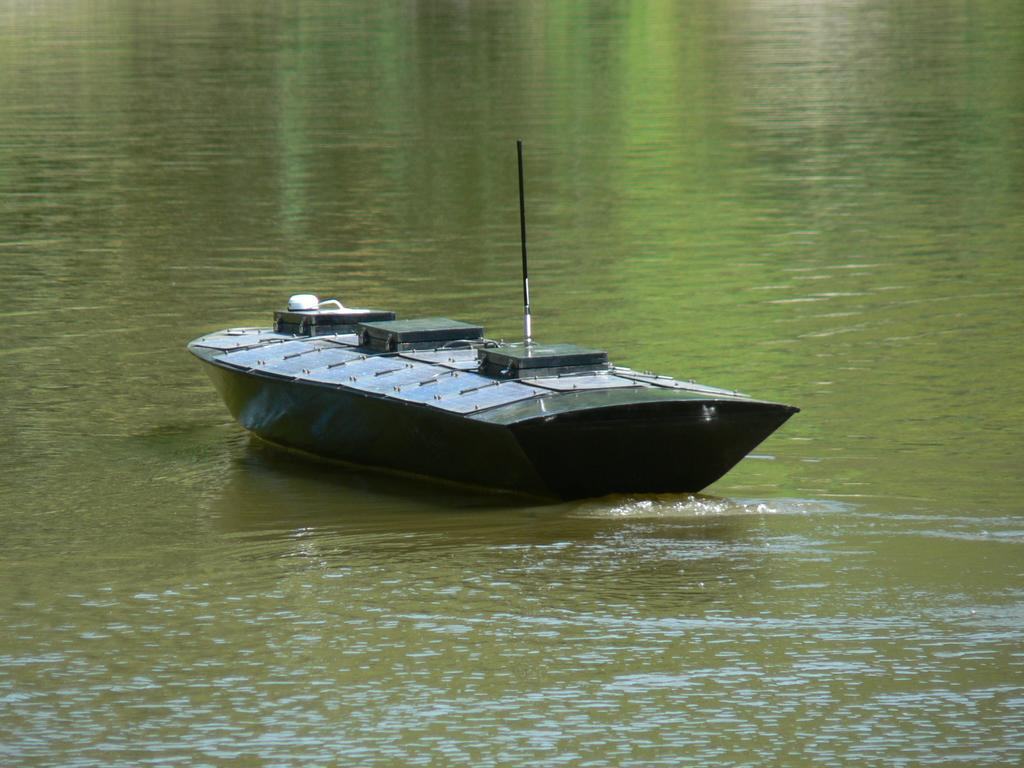
\includegraphics[width=0.75\textwidth,trim={1cm 1cm 1cm 1cm},clip]{img/usv.jpeg}
            \end{block}
        \end{column}
    \end{columns}
\end{frame}  

\begin{frame}{Approach}
    \begin{block}{Heuristics \& Metaheuristics}
        \begin{itemize}
	        \item Analysis and planning techniques are very complex
    	    \item Optimal solutions may take hours or days offline: infeasible online
            \item Human agents able to collect and analyze data without such computations
	        \item \textbf{Heuristic:} using practical measures to achieve a reasonable decision
	        \item \textbf{Metaheuristic:} automatic, indirect heuristic discovery in the form of data-driven, adaptive search strategies
        \end{itemize}
        \begin{center}
            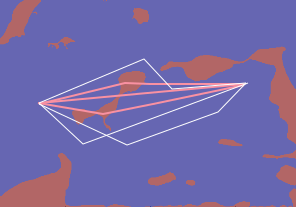
\includegraphics[width=0.5\textwidth,trim={0cm 0cm 0cm 0cm},clip]{img/metaheuristics.png}
        \end{center}
    \end{block}
\end{frame}

\section{System Design}

\begin{frame}{System Design}
    \begin{columns}
        \begin{column}{0.5\textwidth}
            \begin{center}
                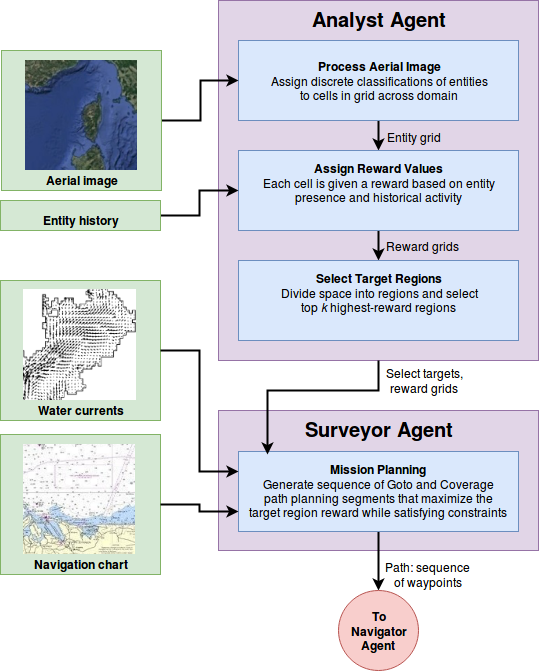
\includegraphics[width=\textwidth,trim={0cm 0cm 0cm 0cm},clip]{img/system_overview.png}
            \end{center}
        \end{column}
        \begin{column}{0.5\textwidth}
            \begin{center}
                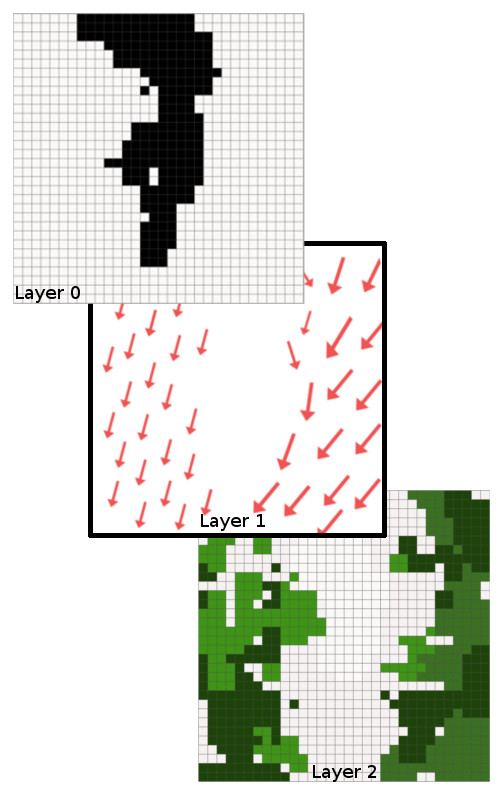
\includegraphics[width=0.75\textwidth,trim={0cm 0cm 0cm 0cm},clip]{img/layers.jpg}
            \end{center}
        \end{column}
    \end{columns}
\end{frame}


\begin{frame}{System Design}
    \begin{block}{Analyst}
        Assigns reward to every cell in region based on entity presence, speed and acceleration
    \end{block}
    \begin{columns}
    
        \begin{column}{0.33\textwidth}
            \begin{columns}
                \begin{column}{0.5\textwidth}
                    \begin{center}
                        %\newline
                        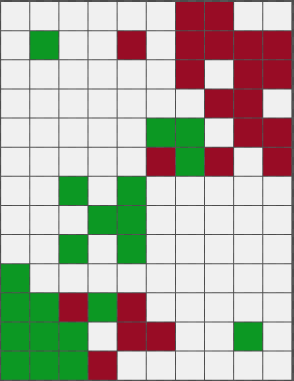
\includegraphics[width=\textwidth,trim={0cm 0cm 0cm 0cm},clip]{img/analyst1.png}
                        \newline
                        Day 1
                        \newline
                        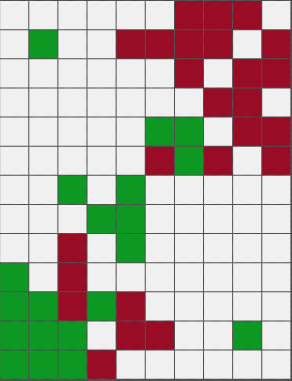
\includegraphics[width=\textwidth,trim={0cm 0cm 0cm 0cm},clip]{img/analyst3.png}
                        \newline
                        Day 3
                    \end{center}
                \end{column}
                \begin{column}{0.5\textwidth}
                    \begin{center}
                        %\newline
                        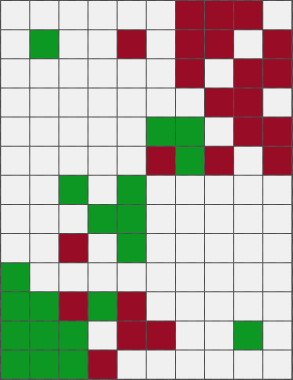
\includegraphics[width=\textwidth,trim={0cm 0cm 0cm 0cm},clip]{img/analyst2.png}
                        \newline
                        Day 2
                        \newline
                        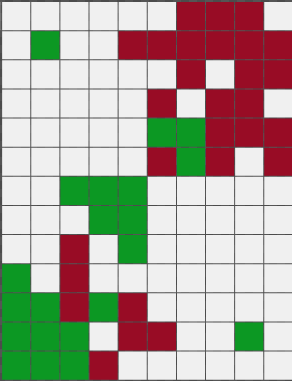
\includegraphics[width=\textwidth,trim={0cm 0cm 0cm 0cm},clip]{img/analyst4.png} 
                        \newline
                        Day 4
                    \end{center}
                \end{column}
            \end{columns}
        \end{column}
        \begin{column}{0.33\textwidth}
            \begin{center}
                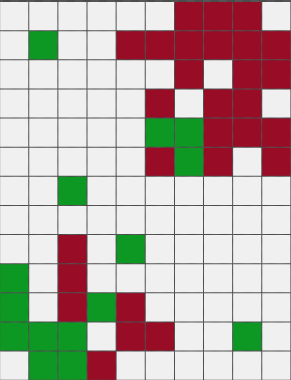
\includegraphics[width=0.50\textwidth,trim={0cm 0cm 0cm 0cm},clip]{img/analyst5.png}
                \newline
                Today's image
                \newline
                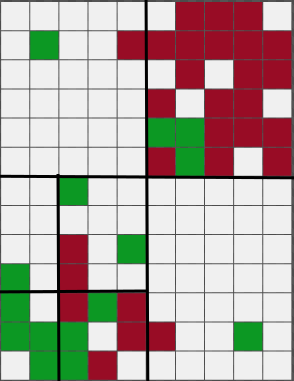
\includegraphics[width=0.50\textwidth,trim={0cm 0cm 0cm 0cm},clip]{img/analyst_grid.png}
                \newline
                Quadtree applied
            \end{center}
        \end{column}
        \begin{column}{0.33\textwidth}
            %\begin{center}
                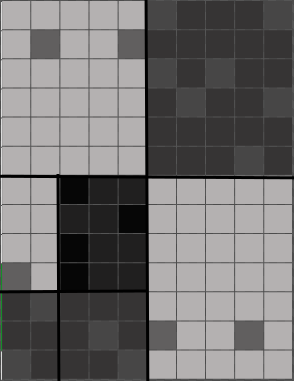
\includegraphics[width=0.50\textwidth,trim={0cm 0cm 0cm 0cm},clip]{img/analyst_grid_2.png}
                \newline
                Reward assignment
                \newline
                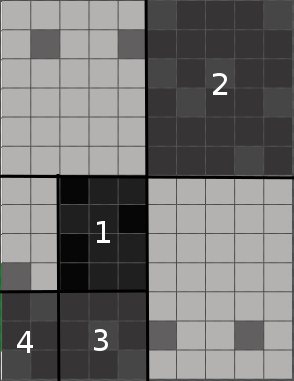
\includegraphics[width=0.50\textwidth,trim={0cm 0cm 0cm 0cm},clip]{img/analyst_grid_targets.png}
                \newline
                Top K targets
            %\end{center}
        \end{column}
    \end{columns}
\end{frame}

\begin{frame}{System Design}
    \begin{block}{Optimality sacrificed for speed}
    \end{block}
    \begin{columns}
        \begin{column}{0.5\textwidth}
            \begin{center}
                \textbf{Quadtree}
                \linebreak
                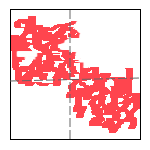
\includegraphics[width=0.75\textwidth,trim={0cm 0cm 0cm 0cm},clip]{img/quadtree_exA.png}
                \begin{itemize}
                        \item Relatively naive
    	                \item Extremely fast
                \end{itemize}
            \end{center}
        \end{column}
        \begin{column}{0.5\textwidth}
            \begin{center}
                \textbf{Optimal}
                \linebreak
                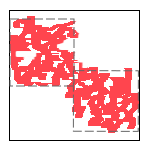
\includegraphics[width=0.75\textwidth,trim={0cm 0cm 0cm 0cm},clip]{img/quadtree_exB.png}
                \begin{itemize}
                        \item Sophisticated reward maximization
    	                \item Very complex
                \end{itemize}  
            \end{center}
        \end{column}
    \end{columns}    
\end{frame}


\begin{frame}{System Design}
    \begin{block}{Surveyer}
        \begin{itemize}
            \item \textbf{Mission planning:} which targets to visit
    	    \item \textbf{\textit{Goto} path planning:} how to get from target to target
    	    \item \textbf{\textit{Coverage} path planning:} how to visit all cells in target region
        \end{itemize}  
    \end{block}
    \begin{columns}
        \begin{column}{0.5\textwidth}
            \begin{center}
                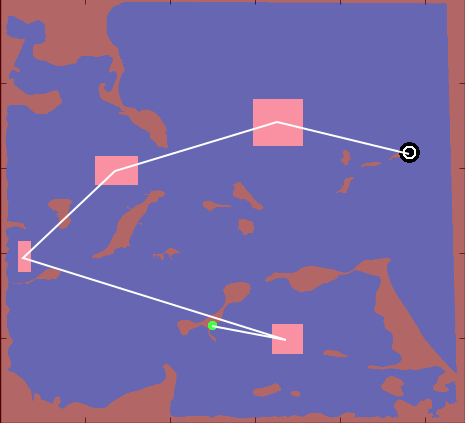
\includegraphics[width=0.75\textwidth,trim={0cm 0cm 0cm 0cm},clip]{img/surveyor_1.png}
                \newline
                Selected target order
            \end{center}
        \end{column}
        \begin{column}{0.5\textwidth}
            \begin{center}
                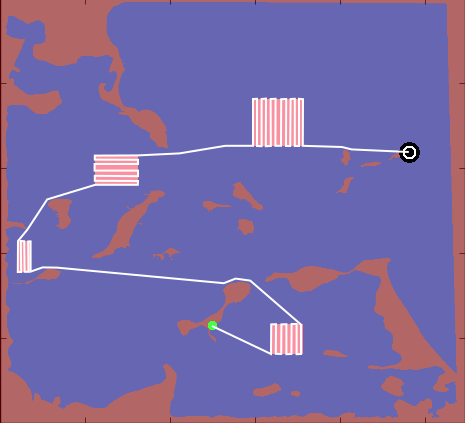
\includegraphics[width=0.75\textwidth,trim={0cm 0cm 0cm 0cm},clip]{img/surveyor_2.png}
                \newline
                \textit{Goto} and \textit{Coverage} paths
            \end{center}
        \end{column}
    \end{columns}
\end{frame}


\begin{frame}{System Design}
    \begin{block}{\textit{Goto} Planning}
        \begin{itemize}
	        \item Optimal is to solve Traveling Salesman Problem (NP-hard)
    	    \item Heuristics are the norm: \textit{A*}, \textit{Potential Field}, \textit{Voronoi Diagram} \newline Still complex for such large regions
            \item Metaheuristics increasingly common: \textit{Genetic Algorithm}, \textit{Particle Swarm Optimization} \newline But nondeterministic and not guaranteed to converge
	        \item Surveyer has to balance opposing criteria
	        \begin{itemize}
	            \item Efficiency: minimize distance, duration, and energy
	            \item Opportunity: maximize reward
	        \end{itemize}
	        \item This work uses metaheuristics. Has to show: 
	        \begin{itemize}
	            \item Approximate optimality
	            \item Acceptable speed and reliability of convergence
	            \item Planning can be modified for a desired behavior
	        \end{itemize}
        \end{itemize}
        %\begin{center}
        %    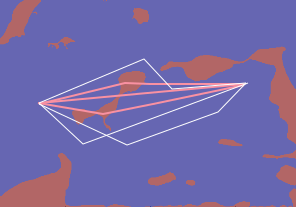
\includegraphics[width=0.5\textwidth,trim={0cm 0cm 0cm 0cm},clip]{img/metaheuristics.png}
        %\end{center}
    \end{block}
\end{frame}

\begin{frame}{System Design}
    \begin{block}{Metaheuristic \textit{Goto} Planning}
        Which algorithm to use? 
	    \begin{itemize}
	        \item Evolutionary approach
	        \begin{itemize}
	            \item Genetic Algorithm (GA)
	            \item Differential Evolution (DE)
	        \end{itemize}
	        \item Colony behavior approach
	        \begin{itemize}
	            \item Particle Swarm Optimization (PSO)
	            \item Artificial Bee Colony (ABC)
	        \end{itemize}
        \end{itemize}
    \end{block}
    \begin{columns}
         \begin{column}{0.5\textwidth}
             \begin{block}{Evolutionary approach}   
                 \begin{center}
                     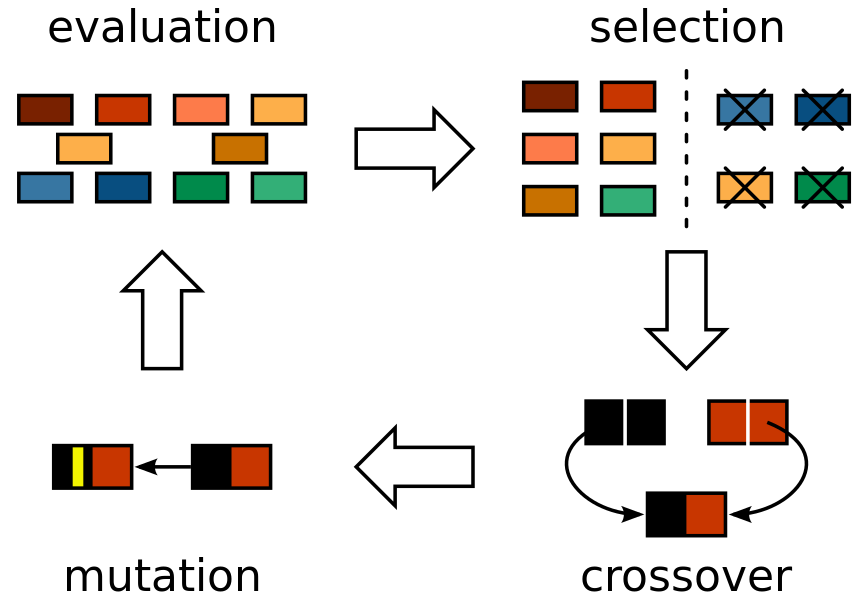
\includegraphics[width=0.8\textwidth,trim={0cm 0cm 0cm 0cm},clip]{img/ga.png}
                 \end{center}
             \end{block} 
        \end{column}
        \begin{column}{0.5\textwidth}
             \begin{block}{Colony behavior approach}   
                 \begin{center}
                     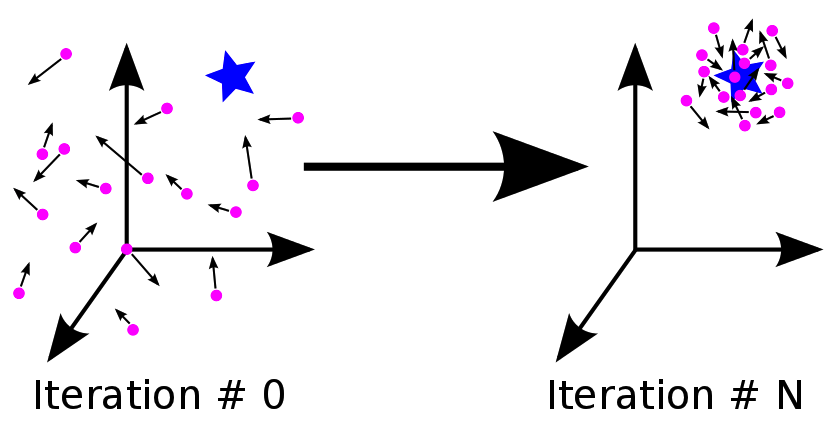
\includegraphics[width=\textwidth,trim={0cm 0cm 0cm 0cm},clip]{img/pso.png}
                 \end{center}
             \end{block} 
        \end{column}
    \end{columns}
\end{frame}

\begin{frame}{System Design}
    \begin{block}{Metaheuristic \textit{Goto} Planning fitness function}
	    \begin{itemize}
	        \item Evaluates an ordered sequence of (row, column) waypoints
	        \item Each cell on the line between each waypoint is evaluated
	        \item Considers multiple weighted criteria
	        \begin{itemize}
	            \item \textbf{Collisions:} number of obstacle cells encountered
	            \item \textbf{Distance:} distance between waypoints
	            \item \textbf{Energy:} applied work done to traverse cell at desired speed and heading
	            \item \textbf{Reward:} reward value at each cell
	        \end{itemize}
	        \item Duration estimate required to index closest temporal water currents forecast
        \end{itemize}
    \end{block}

    \begin{columns}
         \begin{column}{0.33\textwidth}
             \begin{block}{Region}   
                 \begin{center}
                     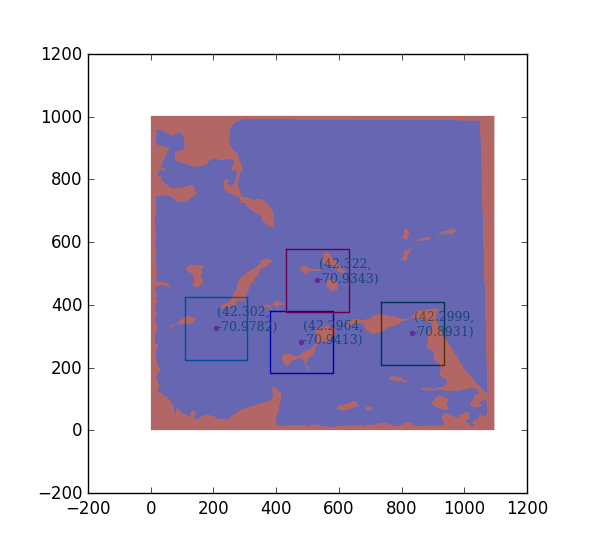
\includegraphics[width=0.8\textwidth,trim={3cm 3cm 3cm 3cm},clip]{img/Fig_targetsMap.png}
                 \end{center}
             \end{block} 
        \end{column}
        \begin{column}{0.33\textwidth}
             \begin{block}{Water currents}   
                 \begin{center}
                     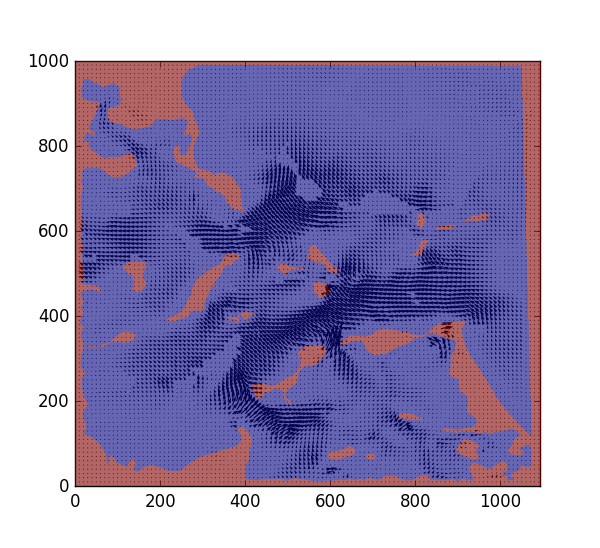
\includegraphics[width=0.75\textwidth,trim={2cm 2cm 1.75cm 1cm},clip]{img/Fig_currentsMap-1.png}
                 \end{center}
             \end{block} 
        \end{column}
         \begin{column}{0.33\textwidth}
             \begin{block}{Entities}   
                 \begin{center}
                     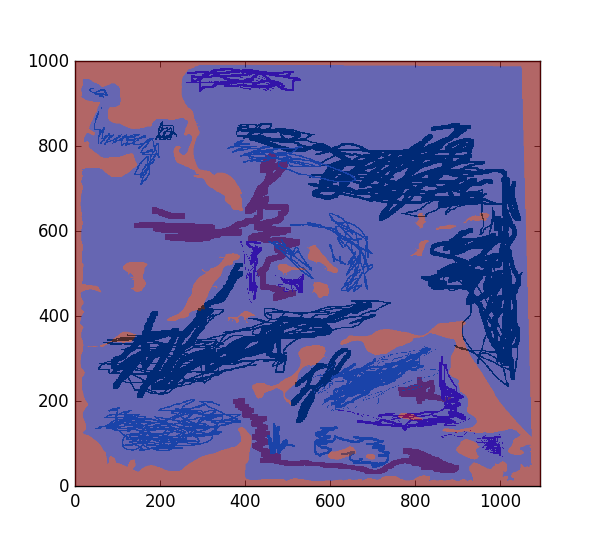
\includegraphics[width=0.75\textwidth,trim={2cm 2cm 1.75cm 1cm},clip]{img/Fig_entitiesMap.png}
                 \end{center}
             \end{block} 
        \end{column}
    \end{columns}


\end{frame}


\section{Evaluation}


\section{Conclusions \& Future Work}

\end{document}
